% Este archivo es parte de la memoria del proyecto fin de carrera
% de Aarón Bueno Villares. Protegida bajo la licencia GFDL.
%
% Para más información, la licencia completa viene incluida en el
% fichero fdl-1.3.tex

% Copyright (C) 2010 Aarón Bueno Villares

\section{Calendario}
\label{sec:calendario}

Aquí se describirá mas concisamente el contenido de cada una de estas
iteraciones de desarrollo.

Hay que advertir que durante todo el tiempo que ha
durado la confección de este proyecto no me he dedicado únicamente al
mismo. Mientras, continuaba las asignaturas que me quedaban de la
titulación técnica y luego comencé a cursar asignaturas del segundo
ciclo. Así que, en muchas ocasiones durante la realización del
proyecto me he visto obligado a pausar el desarrollo del mismo para
dedicarme enteramente a las asignaturas, lo que explica en parte su
larga duración.

En la figura \ref{fig:gantt} se muestra el diagrama de Gantt
correspondiente al calendario de nuestro proyecto.

\subsection{Definición inicial}
Cuando decidí realizar este proyecto, solo tenía una idea vaga de qué
iba a desarrollar. Tenía un propósito y un objetivo, como ya se
advirtió en el capítulo \ref{chap:introduccion}, pero no
sabía de que forma concreta esas ideas tomarían definitivamente
su forma. El primer ciclo de desarrollo corresponde a este periodo de
reflexión inicial, que fecundó en un reglamento que serviría como
punto de partida para el desarrollo consecuente.

En esta iteración se definió la categoría del juego, tras conocer e
investigar los taxones en los que se clasifican los videojuegos, se
conoció algo de la historia del paradigma de juegos de mesa que estaba
implementando para obtener inspiración de diversos reglamentos de
diversos juegos históricos de táctica militar (aunque mi mayor fuente
de inspiración siempre ha sido el reglamento de \emph{WF} por
ser el reglamento que mejor conozco), y se exploró mas concisamente
acerca de si efectivamente mi juego sería el único videojuego de esta
corte, explorando muchas páginas webs dedicadas a la recopilación de
información sobre videojuegos tanto clásicos como modernos. Así que
podemos decir que este primer ciclo también contiene una etapa de
documentación.

También se estuvo decidiendo que \emph{paradigma} de interfaz
usaríamos, si el videojuego sería 3D, isométrico o un juego 2D
plano. Al final me decanté por la última opción, pues no tenía las
artes suficientes para crear los modelos gráficos que necesitaría para
las dos primeras opciones.

Por último, junto a los demás aspectos, se configuró un reglamento
inicial de \gom.

\subsection{Arquitectura general del sistema}
Esta iteración contituye el primer ciclo de diseño, que a su vez es el mas
importante, pues se estableció la arquitectura general del sistema
(véase \ref{sec:diseno}), es decir, como organizaríamos las clases
principales y de mas alto nivel de abstracción que conformarían la
resolución del problema de implementar ese primer reglamento.

\subsection{Fase de movimiento}
La primera fase que se diseñó y luego implementó fue la fase de
movimiento. En su intento de implementación, se rediseñó el reglamento
en gran medida, pues llegé a comprender la gran complejidad que
contenía la versión inicial. Este ciclo contituye casi el 80\% del
desarrollo del sistema, sobre todo por las dificultades en establecer
los cálculos correctos del \emph{gestor de escenarios} (véase
\ref{sec:diseno}), que contenía mucha matemática y geometría.

\subsection{Gestor de interfaz}
Conjuntamente al ciclo anterior, se fue implementando la interfaz
necesaria para poder visualizar las implementaciones del gestor de
movimiento. Esta primera versión del gestor de interfaz fue la que
configuró el aspecto gráfico de las batallas.

\subsection{Fase de combate}
Una vez implementada la fase de movimiento, se podía comenzar a
desarrollar la fase de combate, pues sin la primera, no se podía
desarrollar la segunda (para combatir, hace falta realizar
cargas, cosa que se hace en la fase de movimiento). Nuevamente, el
reglamento sufrió modificaciones en torno a los aspectos involucrados
en esta fase.

\subsection{Mejora de la interfaz}
En esta iteración o ciclo, el gestor de interfaz tomaría su forma
final. Ya no sería un simple \emph{visualizador de batallas}. Ahora
sería una interfaz de menús donde el usuario podía realizar varias
cosas, no solo jugar batallas.

Por ello, se añadió una herramienta para poder configurar ejércitos
desde el propio programa, que luego se podrían elegir desde el mismo
software para comenzar la partida. La creación de esta herramienta
propició una nueva linea de desarrollo que tiene autonomía por sí
misma.

También se dedicó un episodio importante a mejorar
la interfaz gráfica, añadiendo multitud de cambios, a ajustar las
fuentes, las imágenes, los ejércitos y los sonidos, y a realizar
modificaciones en la interfaz para adaptar los nuevos cambios e ideas.

\subsection{Fase de disparos y magia}
En esta iteración, se añadió al juego la fase de disparo, y también se
implementó la magia. La inclusión en el juego de los disparos y la
magia fue bastante sencilla, quizás gracias al buen diseño realizado en las
iteraciones anteriores.

\subsection{Memoria del proyecto}
Una vez terminado de programar el juego, se hizo la memoria del
proyecto. En realidad, esta memoria ya había ido realizándose
paulatinamente junto a las iteraciones anteriores, pero tras finalizar el
juego fue cuando me dediqué enteramente a su confección.

\begin{figure}[h]
  \centering
  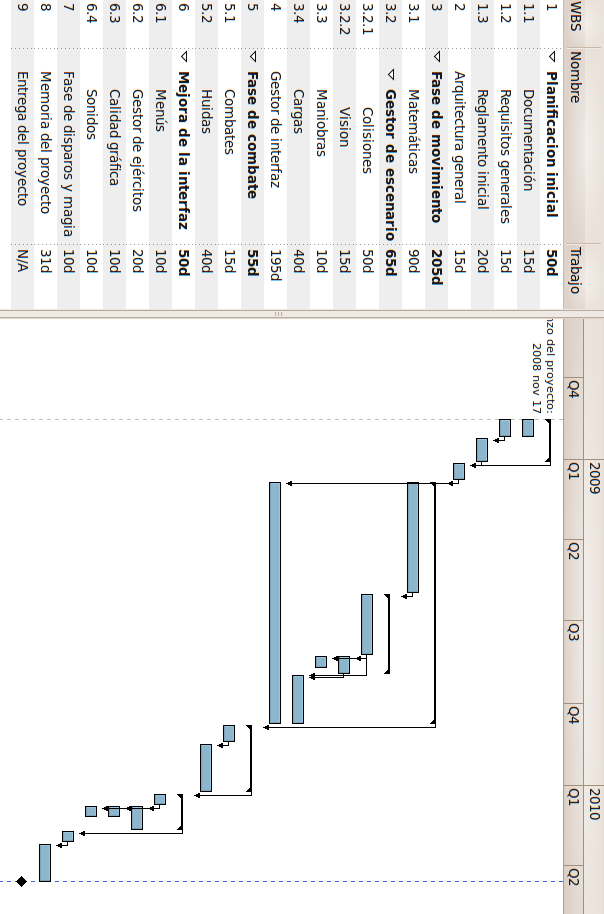
\includegraphics[scale=.5]{./imagenes/Gantt.png}
  \caption{Diagrama de Gantt del calendario del proyecto}
  \label{fig:gantt}
\end{figure}
